\documentclass[11pt]{article}

\usepackage[margin=1in]{geometry}
\usepackage{amsmath}
\usepackage{graphicx}
\usepackage{booktabs}
\usepackage{xcolor}
\usepackage{hyperref}
\usepackage{titlesec}
\usepackage{float}

\titleformat{\section}{\large\bfseries}{\thesection}{1em}{}
\titleformat{\subsection}{\bfseries\color{blue!60!black}}{\thesubsection}{1em}{}

\title{\Large\bfseries MSAI-635 Assignment 1: K-Armed Bandit Problem}
\author{Gaurav Prakash \\ UID: 122250130}
\date{}

\begin{document}

\maketitle

\section{Problem Formulation}
K-armed bandit is a single-state RL problem used to study the
exploration-exploitation tradeoff in isolation. 


At each time step $t$, an agent selects one of $k = 10$ arms (actions). Each arm $a$ has a true, fixed action value $q_*(a)$ drawn once at the start of a run from $\mathcal{N}(0, 1)$. Selecting arm $a$ returns a stochastic reward $R \sim \mathcal{N}(q_*(a), 1)$. The agent does not know $q_*(a)$ and must estimate it online from observed rewards while trying to maximize cumulative reward over 1000 steps. As a result of these unknown true values, the agent faces a fundamental decision at every step: \textbf{exploit the action that currently looks best, or explore other actions to improve
its estimates and potentially find a better one}. 


% Performance is measured with two metrics,
% averaged over 200 independent runs (each with freshly sampled $q_*(a)$): the average reward at
% each step, and the percentage of runs in which the optimal action $a^* = \arg\max_a q_*(a)$
% was selected.

\section{Methodology}

\subsection{Environment and agents}
\texttt{KArmedBandit} (\texttt{bandit.py}) initializes $k$ true action values from
$\mathcal{N}(0, 1)$, exposes \texttt{step(action)} to sample a reward from
$\mathcal{N}(q_*(\text{action}), 1)$, and \texttt{optimal\_action()} to identify the best arm
for scoring purposes only (the agents never see it). Two agents were implemented on top of
this environment, both using incremental sample-average action-value estimates:
\[
Q_{n+1}(a) = Q_n(a) + \frac{1}{N(a)} \left[ R_n - Q_n(a) \right]
\]
\texttt{GreedyAgent} initializes $Q(a) = 0$ for all $a$ and always selects
$\arg\max_a Q(a)$ (ties broken uniformly at random). \texttt{EpsilonGreedyAgent} behaves
identically except that, with probability $\varepsilon$, it selects a uniformly random action
instead of the greedy one. Three settings were evaluated: $\varepsilon = 0.0$ (equivalent to
\texttt{GreedyAgent}), $\varepsilon = 0.01$, and $\varepsilon = 0.1$.

\subsection{Effect of exploration on learning performance}
Because all $Q(a)$ start at zero, the agent's early choices are driven almost entirely by
sampling noise in the first few rewards rather than by the true action values. It directly improves long-run learning
performance: both $\varepsilon$-greedy agents keep raising their \% optimal-action and average-reward curves throughout the full 1000 steps, whereas an agent with no exploration stops learning about arms it has abandoned. The cost of exploration is short-term: every
exploratory step has an expected reward equal to the average of all arms rather than the best one, so more exploration trades away some immediate reward for better long-run action-value
estimates.

\subsection{Why purely greedy action selection can perform poorly}
A purely greedy agent ($\varepsilon = 0$) commits to whichever arm happens to look best after
only a handful of samples. Once an arm's estimate is the highest, the greedy rule keeps
selecting it, which means only that arm's estimate continues to be refined --- every other
arm's estimate is frozen at whatever noisy value it received early on, even if its true value
is higher. 
This is visible directly in our results (Section~4): the greedy agent's \% optimal-action
curve flattens almost immediately, around step 100--200, and stays flat for the remaining
800+ steps because it has stopped gathering any new information.

\subsection{Exploration-exploitation tradeoff}
Exploitation maximizes expected reward given the agent's current (possibly wrong) estimates;
exploration sacrifices some immediate expected reward to gather information that can improve
future decisions. $\varepsilon$ directly parameterizes this tradeoff: $\varepsilon = 0$ is
pure exploitation and risks permanently locking onto a suboptimal arm; a very large
$\varepsilon$ would be almost pure exploration and would rarely capitalize on what it learns, capping a lower average reward even after identifying the optimal arm. A small, nonzero value for $\varepsilon$ strictly dominates pure
greedy action selection in this experiment.

\section{Experimental Setup}
Each of the three agents (Greedy, $\varepsilon$-greedy with $\varepsilon = 0.01$,
$\varepsilon$-greedy with $\varepsilon = 0.1$) was evaluated on a $k = 10$ armed bandit for
1000 time steps per run, averaged over 200 independent runs
Implementation: Python 3, NumPy for sampling and vectorized averaging, Matplotlib for plotting
(\texttt{bandit.py}, \texttt{agents.py}, \texttt{experiment.py}). At each checkpoint step, the
average reward and percentage of optimal-action selections across the 200 runs were recorded


\begin{table}[h]
\centering
\begin{tabular}{c cc cc cc}
\toprule
Step & \multicolumn{2}{c}{Greedy} & \multicolumn{2}{c}{$\varepsilon=0.01$} & \multicolumn{2}{c}{$\varepsilon=0.1$} \\
\cmidrule(lr){2-3} \cmidrule(lr){4-5} \cmidrule(lr){6-7}
 & Avg R & \% Opt & Avg R & \% Opt & Avg R & \% Opt \\
\midrule
1    & -0.08 & 8.0\%  & 0.08 & 12.5\% & -0.08 & 9.0\%  \\
10   & 0.80  & 24.5\% & 0.90 & 33.0\% & 0.84  & 29.5\% \\
50   & 1.00  & 30.5\% & 1.05 & 38.0\% & 1.14  & 45.0\% \\
100  & 1.01  & 32.5\% & 0.96 & 40.5\% & 1.28  & 58.0\% \\
200  & 0.93  & 32.5\% & 1.17 & 47.0\% & 1.36  & 67.5\% \\
500  & 1.06  & 32.5\% & 1.37 & 53.0\% & 1.58  & 77.5\% \\
1000 & 1.03  & 32.5\% & 1.33 & 58.0\% & 1.32  & 81.0\% \\
\bottomrule
\end{tabular}
\caption{Average reward and \% optimal-action selection at checkpoint steps, averaged over 200 runs.}
\end{table}

\clearpage
\section{Plots}

\begin{figure}[H]
\centering
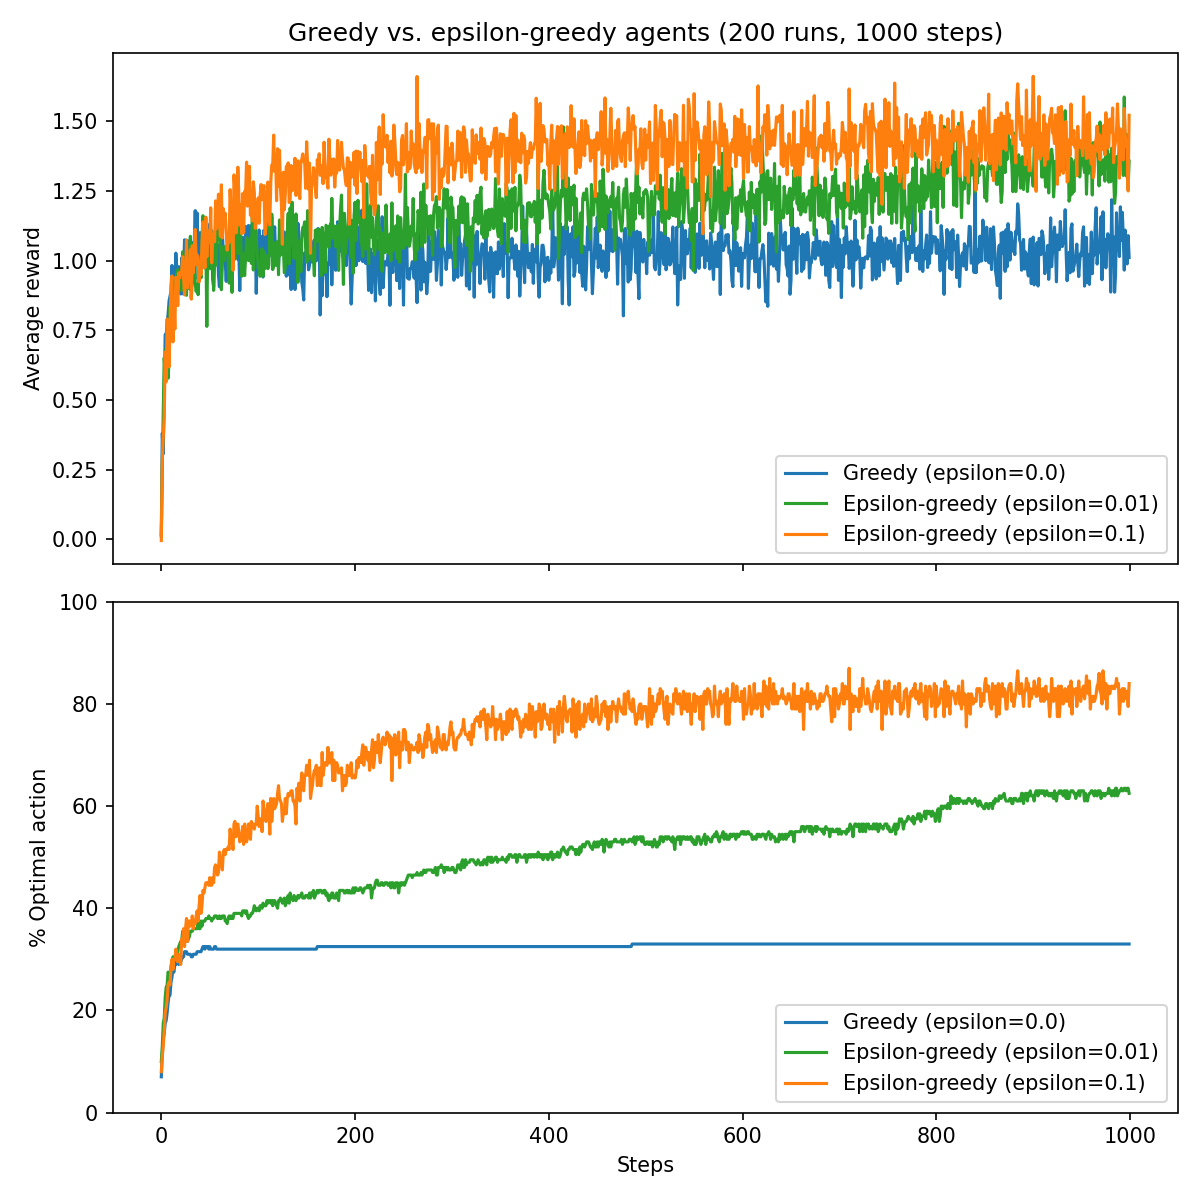
\includegraphics[width=\textwidth]{epsilon_greedy_agent_performance.png}
\caption{Average reward (top) and \% optimal-action selection (bottom) vs. time step, for
Greedy ($\varepsilon=0.0$), $\varepsilon$-greedy ($\varepsilon=0.01$), and $\varepsilon$-greedy
($\varepsilon=0.1$), each averaged over 200 independent runs of 1000 steps.}
\end{figure}

\clearpage
\section{Discussion}

\subsection{Comparison of epsilon values}
The three agents separate clearly on both metrics. Greedy ($\varepsilon = 0.0$) rises fastest
in the first 50 steps but then plateaus almost completely: \% optimal action
flattens at 32.5\% and average reward stalls around 0.9--1.1 for the rest of the
run, since the agent stops exploring once an early estimate looks best. $\varepsilon$-greedy
with $\varepsilon = 0.01$ explores rarely, so it improves slowly but steadily, still climbing
at step 1000 (58.0\% optimal action, average reward 1.33)
without having converged. $\varepsilon$-greedy with $\varepsilon = 0.1$ explores far more
aggressively and consequently identifies the optimal arm much faster, reaching
81.0\% optimal action and the highest average reward
(1.32--1.58 in the later steps) within the 1000-step budget.

\subsection{Which epsilon performed best, and why}
Within this experiment's 1000-step horizon, $\varepsilon = 0.1$ performed best, achieving both
the highest average reward and the highest \% optimal-action rate throughout most of the run.
It performs best because it explores often enough to sample all 10 arms thoroughly within just
a few hundred steps, letting its $Q(a)$ estimates converge to the true $q_*(a)$ values
quickly; once converged, it still exploits the identified best arm 90\% of the time, which is
frequent enough to translate that accurate knowledge into high reward within a short horizon.
$\varepsilon = 0.01$ is not worse in principle --- given a much longer horizon (many thousands
of steps), it would eventually match or exceed $\varepsilon = 0.1$'s average reward, because
once it also identifies the best arm it wastes only 1\% of steps on random exploration versus
10\% --- but within the 1000 steps tested here it simply has not explored enough yet to catch
up. Pure greedy ($\varepsilon = 0.0$) performs worst of all three because it has no mechanism
to correct an early mistake.

\section{Conclusions}
This experiment confirms the classic exploration-exploitation result for the k-armed bandit:
some exploration is necessary for reliable learning, but the right amount depends on the time
horizon available. Purely greedy action selection converges quickly but is structurally prone
to locking onto a suboptimal action, since it never revisits arms it has already dismissed ---
it was the worst performer of the three by a wide margin on both metrics. Introducing a small,
constant probability of exploration ($\varepsilon$-greedy) fixes this by continually
refreshing action-value estimates, at the cost of some reward being spent on exploratory,
non-greedy actions. That cost is precisely the exploration-exploitation tradeoff: more
exploration ($\varepsilon = 0.1$) finds the optimal arm faster and won this 1000-step
comparison, while less exploration ($\varepsilon = 0.01$) wastes less reward long-term but
needs a much longer horizon to pay off.

\end{document}
